%
% File acl2015.tex
%
% Contact: car@ir.hit.edu.cn, gdzhou@suda.edu.cn
%%
%% Based on the style files for ACL-2014, which were, in turn,
%% Based on the style files for ACL-2013, which were, in turn,
%% Based on the style files for ACL-2012, which were, in turn,
%% based on the style files for ACL-2011, which were, in turn, 
%% based on the style files for ACL-2010, which were, in turn, 
%% based on the style files for ACL-IJCNLP-2009, which were, in turn,
%% based on the style files for EACL-2009 and IJCNLP-2008...

%% Based on the style files for EACL 2006 by 
%%e.agirre@ehu.es or Sergi.Balari@uab.es
%% and that of ACL 08 by Joakim Nivre and Noah Smith

\documentclass[11pt]{article}
\usepackage{acl2015}
\usepackage{times}
\usepackage{url}
\usepackage{latexsym}
\usepackage{todonotes}

\usepackage{amsmath}
\usepackage{booktabs}
\usepackage{amssymb}
\setcounter{tocdepth}{3}
\usepackage{graphicx}
\usepackage{caption}
\usepackage{url}

\usepackage[ruled,vlined]{algorithm2e}
\include{pythonlisting}

\DeclareMathOperator*{\argmax}{arg\,max}

\usepackage{gb4e}
\noautomath

\usepackage{array,multirow}

\usepackage{array}
\newcolumntype{L}[1]{>{\raggedright\let\newline\\\arraybackslash\hspace{0pt}}m{#1}}
\newcolumntype{C}[1]{>{\centering\let\newline\\\arraybackslash\hspace{0pt}}m{#1}}
\newcolumntype{R}[1]{>{\raggedleft\let\newline\\\arraybackslash\hspace{0pt}}m{#1}}

\usepackage{arabtex}
\novocalize
\setfarsi
\yahnodots

\hyphenation{RelAgg}
\hyphenation{RelGreedy}

%\setlength\titlebox{5cm}

% You can expand the titlebox if you need extra space
% to show all the authors. Please do not make the titlebox
% smaller than 5cm (the original size); we will check this
% in the camera-ready version and ask you to change it back.


\title{Unsupervised Cross-Lingual Word Sense Disambiguation on Languages with Scarce Resources: Application to Persian}

\author{}

\date{}

\begin{document}
\maketitle
\begin{abstract}
\vspace{-0.2cm}
We explore the use of unsupervised methods in Cross-Lingual Word Sense Disambiguation (CL-WSD) with the application of English to Persian (Farsi). We create a new test collection for CL-WSD in Persian, following the format of the SemEval 2013 CL-WSD task. We then evaluate our semantic vector word representation-based approach on the new evaluation benchmark and compare it with the standard baseline of the task as well as the state-of-the-art unsupervised system (CO-Graph). The results show that our approach outperforms both the standard baseline and the CO-Graph system in both of the task evaluation metrics (\emph{Out-Of-Five} and \emph{Best result}).
\vspace{-0.2cm}
\end{abstract}


\section{Introduction}
\vspace{-0.2cm}
\label{sec:introduction}
Word Sense Disambiguation (WSD) is the task of automatically  selecting the most related sense for a word occurring in a context. WSD is considered as a main step in the course of approaching language understanding beyond the surface of the words and has been intensively studied in Natural Language Processing (NLP)~\cite{navigli2012quick}. WSD is used in Machine Translation~\cite{chan2007word,costa2014statistical}, Information Retrieval~\cite{zhong2012word,na2011enriching}, or Entity Linking~\cite{moro2014entity}.

Typically, the methods for approaching WSD are classified into knowledge-based, supervised, and unsupervised. Knowledge-based approaches use available structured knowledge% and apply algorithms by considering the structural and the connectivity properties of the model
~\cite{agirre2014random,miller2012using}. Often, the systems exploit WordNet~\cite{fellbaum1998wordnet} as the sense inventory, together with graph-based methods~\cite{agirre2010graph,guo2010combining}.
Supervised approaches learn a computational model based on large amounts of annotated data. While these two approaches show competitive results in practice, they both have to face the knowledge acquisition bottleneck. This is a particular problem in specific domains or scarce-resource languages~\cite{pilehvar2014large}. As an alternative, unsupervised approaches address WSD using only information extracted from existing corpora, such as various term co-occurrence indicators~\cite{di2013clustering}.

As a paradigm, multilingual and cross-lingual WSD focus on lexical substitution in a target language. The creation of large knowledge resources such as BabelNet~\cite{navigli2010babelnet} and DBPedia~\cite{auer2007dbpedia} have opened up new possibilities for solving these tasks with multilingual data. For example, Navigli and Ponzetto~\shortcite{navigli2012joining} exploit BabelNet to develop their graph-based monolingual and bilingual WSD across main European languages.

Cross-lingual Word Sense Disambiguation (CL-WSD) targets disambiguation of one word in a source language while translating to a target language. SemEval-2010~\cite{lefever2010semeval} and SemEval-2013~\cite{lefever2013semeval} provide an evaluation platform for term disambiguation  from English to Dutch, German, Italian, Spanish, and French. % The participating systems mostly exploit the Europarl corpus~\footnote{\url{http://www.statmt.org/europarl/}}, a domain specific parallel corpora. For instance, Levefer~\shortcite{lefever2011parasense}, Rudnick et al.~\shortcite{rudnick2013hltdi}, and Gompel et al.~\shortcite{gompel2013wsd2} align the words in the parallel corpus and then follow classification-based approaches on the context features, while Silberer et al.~\shortcite{silberer2010uhd} exploit the connection between nodes after building a multilingual co-occurrence graph. 
As the task introduces the Europarl corpus~\cite{europarl} as the main resource, many participating systems exploit these parallel corpora to overcome the knowledge acquisition bottleneck~\cite{lefever2011parasense,rudnick2013hltdi}. However, these methods are not applicable for many languages and domains due to the scarcity of bilingual corpora. Persian, for instance, suffers from the lack of reliable and comprehensive knowledge resources as well as parallel corpora. In such cases, unsupervised methods based on monolingual corpora (together with bilingual lexica) are preferable, if not the only available option~\cite{sofianopoulos2012implementing}. %Generally, such methods are based on monolingual corpora in combination with bilingual lexica~\cite{sofianopoulos2012implementing}. 
For example, Bungum et al.~\shortcite{bungum2013improving} find the probable translations of a context in the source language and identify the best using a language model of the target language. Duque et al.~\shortcite{duqueco} build a co-occurrence graph in the target language, and test a variety of graph-based algorithms for identifying the best translation match.

In terms of combining WSD and Semantic Vector Representations of words, Chen et al.~\shortcite{chen2014unified} use knowledge-based WSD to identify distinct representations for different senses of the same term. Our approach for CL-WSD is the opposite of this: starting from general vector representations of terms, it identifies their different senses in context. %mainly based on the relation between semantic vector representation of the words in the target language.  
As vector representations we used two state-of-the-art methods: Word2Vec and GloVe. Word2Vec~\cite{mikolov2013efficient} introduces a highly incremental and scalable method such that when trained on large datasets, it makes it possible to capture many linguistic subtleties (e.g. similar relation between Italy and Rome in comparison to France and Paris). More recently, GloVe~\cite{pennington2014glove} shows superior results in exploiting the implicit knowledge within corpora. 

%We target the problem of CL-WSD from English to Persian language using an unsupervised solution based on vector representation of the words.
In order to evaluate our system, following the format of SemEval CL-WSD task~\cite{lefever2013semeval}, %we created and make available a new test collection for Persian. In fact, 
we contributed Persian as a new language to the framework of the task by providing a new test collection. We compared our approach and the CO-Graph system~\cite{duqueco} on this new evaluation collection, observing the advantages of using vector representations in WSD.

The contributions of the work are two-fold:
\vspace{-0.2cm}
\begin{enumerate}
\item Creating a new CL-WSD benchmark for Persian.
\vspace{-0.2cm}
\item Providing a new state-of-the-art for unsupervised CL-WSD methods, based on the use of vector representations of words.
\end{enumerate}
\vspace{-0.2cm}

The remainder of this paper is organized as follows: Section~\ref{sec:relatedwork} investigates the available Persian language resources. Section~\ref{sec:persian_collection} describes in detail the creation of the new Persian CL-WSD evaluation task. Then, Section~\ref{sec:methodology} explains our unsupervised approach to solve the introduced task, followed by the outline of our experiments in Section~\ref{sec:experiments}. %Results are finally concluded in Section~\ref{sec:conclusion}.

\vspace{-0.2cm}

\section{Resources in Persian Language}
\vspace{-0.2cm}
\label{sec:relatedwork}
Persian is a member of the Indo-European language family, and uses Arabic letters for writing. %The language has a rich morphology system and also many complexities in orthography. 
Seraji et al.~\shortcite{seraji2012} provide a comprehensive overview on the main characteristics of the language. %For example, they show how the word ``the libraries'' can be written in up to 12 different writing styles. 
For instance, the diacritic signs are not written---it is expected that the reader can read the text in the absence of the short vowels. This characteristic causes a special kind of word ambiguity in writing, such that some words are pronounced differently while their written forms are the same e.g., \<k^sty> ``wrestling'' and ``ship''.

%\paragraph{Orthography} Among other languages, Persian is a language with challenging preprocessing tasks. Persian writing is based on Arabic letters plus foura additional ones:. In Persian characters have different forms depending on their position in the word. Based on how they connect to eacht other, there are two categories \cite{seraji2012}: 1) dual-joining: Characters have two different shapes based on their position in the sentence like sin  2) right-joining: These characters do not accept any character from left-hand side like r, z in norouz. Further, in Persian languages we have semi-spaces (zero-width non-joiner spaces). In case of wrong usage, this causes disambiguity. For instance "daarabaad" meaning a known place in Tehran, which with regular spaces means a built place. This causes errors in correct processing of NLP tools.

%\paragraph{Morphological difference} There is no grammatical gender for suffixing affixational morphology of Persian language \cite{amtrup2000}. With adjectives, a suffix is added to the adjective indicating its comparative (adding tar) or superlative forms (adding tarin). For instance for adjective sard (cold), we have sard-tar and sardtarn. In nouns, the plural form is made by adding ha or an to the noun like derakht (tree) and derakhtha or derakhtan. Comparable to 'a/an' in English, Persian has  (ie) which give the meaning of one: derakhti (one three). In verbs, are used to convey tenses, mood and subject. Usually the past tense has the same stem of the verb, and by adding another verb the future form is made, e.g, mikhoram, khordam, khaham khord. Negation is made by adding n (not) at the beginning of the verb, keeping the verb as one word. However, when it comes to compound verbs, the constructions are mostly irregular (combination of nouns and adjectives). 

%Saedi et al.\cite{saedi2009} propose an automatic Persian/English translator containing two modules for En to Pr and Pr to En translation. To perform WSD in the first module, they extend the Lesk algorithm~\cite{lesk1986automatic} by assigning different scores to the words in the gloss. In Lesk algorithm, neighborhood  of a word is assumed to share a common topic with the word. In scoring they consider POS ad sense tags of each word. They utilize combination of rule-based and semantic methods to improve the result.  An important catalog to extend the word structures is WordNet, which groups English words with structured sets. 
 
In recent years, several tools and libraries were introduced, targeting the complexities of Persian language in NLP. For example, Seraji et al.~\shortcite{seraji2012} provides a set of tools for preprocessing (Pre-Per), sentence segmentation and tokenization (SeTPer), and also POS tagging (TagPer). Dehdari et al.~\shortcite{dehdari2008link} brings forward a stemmer and morphological analyzer, called PerStem. More recently, Samvelian et al.~\shortcite{samvelian2014extending} introduces PersPred, focusing on processing of compounding verbs. Finally, Feely et al.~\shortcite{feely2014cmu} provides a front-end and new tools for language processing. In this work, similar to Jadidinejad et al.~\shortcite{jadidinejad2010evaluation}, we use PerStem for stemming, together with TagPer as a state-of-the-art POS tagging tool.

In addition to the NLP tools, knowledge and data resources are an important part of WSD and CL-WSD solutions. The main knowledge resource in Persian is \emph{FarsNet}~\cite{shamsfard2010semi}---the Persian WordNet. Its structure is comparable to WordNet and goes by the same principles while containing significantly fewer words ($\sim$13K versus $\sim$147K). Also, most of its synsets are mapped to synsets in WordNet using equal or near-equal relations.%, resulting in connection between Persian and English synsets. 

While the knowledge-based systems are limited %to the borders of the knowledge resource and not 
and only at high cost extendable to more specific domains, exploiting  parallel corpora can be another effective method for CL-WSD. The existing parallel corpora (English-Persian) are as follows: Tehran English-Persian Parallel (TEP) ~\cite{pilevar2011tep} corpus---a free collection extracted from 1600 movie subtitles. The Parallel English-Persian News (PEN)~\cite{farajian2011pen} corpus aligns 30K sentences of news corpora. However, to the extent of our knowledge, this collections is not yet available. Finally, the collection provided by European Language Resource Association (ELRA) which is a commercial collection with approximately 100K aligned sentences. Among the mentioned resources, TEP is the only publicly available one, but it only contains informal conversations, and therefore it does not provide a general representation of the language.% for NLP solutions. 

In the absence of reliable and comprehensive resources, our unsupervised CL-WSD method exploits the use of monolingual corpora. The available text collections in Persian are as follows: The \emph{Hamshahri} collection~\cite{aleahmad2009hamshahri}, a widely used Persian collection, containing approximately 318K news articles of the Hamshahri newspaper. The articles are of various subjects of economy, sport, politics, psychology, literature, or art from 1996 to 2007. The collection was introduced as the main resource for the Persian task of the CLEF Ad Hoc track~\cite{ferro2010clef,agirre2009clef} in 2008/2009. The \emph{dotIR} collection\footnote{\url{http://ece.ut.ac.ir/DBRG/webir/index.html}}, released in 2008, is created by crawling ~1000K web pages in the .ir domain. Finally,  \emph{Bigjekhan}\footnote{\url{http://ece.ut.ac.ir/dbrg/Bijankhan}} and Uppsala Persian Corpus (UPEC)~\cite{seraji2012} are smaller collections with manually tagged POS data. 

Between the Hamshahri and dotIR (as bigger collections), since the Hamshahri collection is more recent and  has also been used more in the community of Information Retrieval (IR) and NLP, we selected it as the main resource for our experiments. In addition, in comparison to the dotIR collection, as the content of the Hamshahri collection contains revised newspaper articles, we assume that it is a better representation of the language. 

%The task is based on Hamshahri collection~\cite{aleahmad2009hamshahri} with size of 700 MB and 160,000 documents with various topics.

In terms of related work addressing the CL-WSD problem in Persian, Sarrafzadeh et al.~\cite{sarrafzadeh2011} follows a knowledge-based approach by exploiting FarsNet together with leveraging English sense disambiguation. %Their model consists of three phases of: English sense disambiguation, utilizing WordNet and FarsNet to transfer the sense, and selecting the sense from FarsNet. As another method, they investigate direct WSD by applying extended Lesk algorithm~\cite{lesk1986automatic} for Persian WSD. They count the number of shared words between two glosses, the gloss of each sense of the target word with the gloss of other words in the phrase. The one with larger number of common words is chosen. 
%They test on parallel page of Wikipedia in English and Persian evaluated by experts. %Finally, they show that the first approach works better since they can use the state of the art disambiguater of English language and direct approach suffers from lack of NLP tools and ambiguity of Farsi words. 
However, since they evaluate their methods only internally, the results are impossible to compare with other possible approaches. %This lack of standard and reproducible evaluation in Persian, especially in the NLP and MT domain can be seen in other work~\cite{motazedi2009english}. 
%mihai:perhaps add back this last sentence if space allows, but it doesn't say much.

In this work, we address this shortage by creating a new CL-WSD benchmark  for Persian, based on the SemEval 2013 CL-WSD task. We then report the result of our unsupervised approach on the provided benchmark and compare it with a state-of-the-art CL-WSD system.
\vspace{-0.2cm}

\section{Persian CL-WSD Evaluation Benchmark}
\vspace{-0.2cm}
\label{sec:persian_collection}
In this section, we describe in detail the process of creating the CL-WSD evaluation benchmark from English to Persian. The created test collection completely matches the output format of the SemEval 2013 CL-WSD task~\cite{lefever2013semeval} and in fact adds a new language to this multilingual task. In addition, we tightly follow the methods in this task for the creation of the gold standard, with only minor alterations necessary in view of the available Persian language resources.    

\vspace{-0.2cm}
\subsection{SemEval 2013 CL-WSD}
The SemEval 2013 Cross-lingual Word Sense Disambiguation task aims to evaluate the viability of multilingual WSD on a benchmark lexical sample data set. Participants should provide contextually correct translations of English ambiguous nouns into five target languages: German, Dutch, French, Italian, and Spanish. The task contains a test set of 20 nouns, each with 50 sentences. 

%The gold standard of the task is based on the Europarl parallel corpus~\cite{europarl}, and on a collection of English sentences entailing lexical sample words, annotated with their appropriate translations.

In order to create the golden standard as described in Lefever et al.~\shortcite{lefeverparallel}, in the first step a sense inventory was constructed based on the possible translations of the ambiguous terms. In order to find the target translations, they ran word alignment on aligned sentences of the Europarl Corpus~\cite{europarl} and manually verified the results. In the next step, the resulting translations were clustered by meaning per focus words. Finally, annotators used this clustered sense inventory to select the correct translation for each word, for up to three translations per word. %If none of the translations was appropriate, they were allowed to chose . 

Two different evaluation methods are used for the task: 1) \emph{Best Result} evaluation, in which the system suggests any number of translations for each target word%that system results to be correct
, and the final score is divided by the number of these translations. 2) \emph{Out-of-five} (OOF) or more relaxed evaluation, in which the system provides up to five different translations, and the final score is that of the best of these five (more details in Lefever et al.~\shortcite{lefever2013semeval}).

\vspace{-0.2cm}
\subsection{New Persian Collection} 
Similar to Lefever et al.~\shortcite{lefeverparallel}, the creation of CL-WSD task for  Persian  consists of two parts: 1) Creating the sense inventory and 2) Annotation of the translations (i.e. the ground truth).

To create the sense inventory for the 20 nouns, due to the lack of a representative parallel corpora, we leveraged three main dictionaries of the Persian language---Aryanpour, Moein, and Farsidic.com---to obtain as large a coverage as possible for their translations. The translations themselves were added by a Persian linguist.

In order to provide a thorough set of translations, in addition to different meanings of nouns,  their idiomatic meanings (in combinations) are also considered. For example, for the word ``pot'', a wide variety of direct translation (\<gldAn>, \<dyg>, \<qwry>, \<ktry>) were selected. However, there is an expression like ``melting pot''%(A place or situation in which different people and cultures get mixed)
, which is not in the dictionaries. These idiomatic meanings were added  to the senses of this word as an expression or equal idiom, which in this case is \<jAm`h\hspace{0ex}y ^cnd n^zAdy>.

The linguist also divided the translations into different senses.% with related translations.
The resulting clusters for nouns range from 2 (e.g., ``education'' to \<t.h.syl> or \<m`rft>) to 6 clusters (e.g., ``post'' to \<pst>, \<mqAm>, \<m.hl mAmwryt>, \<tyr `mwdy>, \<rAy gyry>, \<m`ny A.s.tlA.hy>). The number of translations ranged from 13 for the word ``mood'' to 42 for the word ``ring''\footnote{Available at resources/sense-inventory}. Table~\ref{tbl:statistics} shows details of these statistics.

\begin{table}[t!]
\footnotesize
\caption{Overview of annotators consensus for Persian language}
\vspace{-0.2cm}
\begin{tabular} {c C{0.7cm} C{0.7cm} C{1.3cm} C{1.5cm} }\hline
word  & \# of clus. & \# of trans. & avg. \# clus./sent. & \% clus. consensus \\
\hline\hline
coach&4 &18 & 1.00 & 98 \\\hline
education&2 &15 & 1.02 & 98 \\\hline
execution& 3&14 & 1.08 & 92 \\\hline
figure  &5 & 33& 1.08 & 92 \\\hline
job &3 & 21& 1.02 & 98 \\\hline
letter &4 & 29& 1.04 & 96 \\\hline
match   &3 &19 & 1.04 & 96 \\\hline
mission &3 & 19& 1.02 & 98 \\\hline
mood    & 2& 13& 1.00& 100 \\\hline
paper   & 3& 32& 1.02 & 98 \\\hline
post    & 6& 38& 1.00 & 100 \\\hline
pot     & 4& 34& 1.04 & 96 \\\hline
range   &5 & 36& 1.04 & 96 \\\hline
rest    & 4&40 & 1.00 & 100 \\\hline
ring    & 6& 42& 1.04 & 98 \\\hline
scene    & 4&25 & 1.02 & 98 \\\hline
side     & 3& 32& 1.00 & 96 \\\hline
soil     & 3& 18& 1.00 & 100 \\\hline
strain	& 4& 39& 1.02 & 98 \\\hline
test& 2& 13& 1.00 & 100 \\\hline  
\end{tabular}
\label{tbl:statistics}
\vspace{-0.5cm}
\end{table}

In a second phase, this generated sense inventory is used to annotate the sentences in the test set (50 sentences for each ambiguous word). This phase was performed by three Persian native-speakers. Via a web-based application\footnote{Available at software/webapplication}, annotators choose the appropriate translations in two steps: In the first step, they choose the related sense (cluster). In the second step, the system showed the related translations for the sense, of which they choose up to three translations. In case of no related translation, they choose nothing and continued to the next question. The agreement between annotators is shown in Table~\ref{tbl:statistics} and is similar to that observed by Lefever et al.~\shortcite{lefeverparallel}.

Using the annotated data, we created the gold standard\footnote{Available at resources/golden} in the same format as Lefever et al.~\shortcite{lefever2013semeval}, such that all the evaluation scripts used in the SemEval 2013 CL-WSD task can also be used on this data. Example~\ref{ex:golden1} and Example~\ref{ex:golden2} show the ground truth for two sentences with the word ``coach'':

\begin{exe}
	\ex SENTENCE 2: A branch line train took us to where a \emph{coach} picked us up for the journey up to the camp.\\
      coach.n.fa 2 :: \<Atwbws> 3; \<Atwmbyl> 2; \<wAgn> 1;
\label{ex:golden1}
\end{exe}
\begin{exe}
    \ex SENTENCE 16: Agassi's \emph{coach} came to me with the rackets.\\
        coach.n.fa 16 :: \<mrby> 3; \<mrby wrz^s> 2; \<srmrby> 2; \<m`lm x.sw.sI> 1;
\label{ex:golden2}
\end{exe}


\vspace{-0.2cm}

\section{Unsupervised CL-WSD Method}
\vspace{-0.2cm}
\label{sec:methodology}
In this section, we introduce our unsupervised approach for Cross Lingual Word Sense Disambiguation. The approach follows the main idea of the Lesk algorithm~\cite{lesk1986automatic}, namely that words in a given context tend to share a common topic. % or, in other words tend to be more similar from semantics point of view. 
 In the absence of external knowledge sources, we use the terms' vector representations to compute their semantic similarity. %In this approach, first using a big corpus, vector representation of the words is created and then using a distance function (i.e. Cosine) the distance between the vectors is computed.   
%Considering the translation of the words in the source language to a group of words in the target language, 
%We apply the mentioned idea to CL-WSD by 
We measure the relatedness of each possible translation of the ambiguous word to all possible translations of the words in its context and select the one that is most similar to the context. %For the translation, we first use a bilingual lexicon %to translate all the words in the source language to all of their possible translations. 
%we use a public online translation API.

To formulate our approach, let us define the list $T$ of translation sets for the words in the context: $T=\{{T_1,T_2,..,T_n} \}$ where $n$ is the number of words in the context, and $T_i$ is the set of translations for the $i^{th}$ word in the context. For each possible translation $t\in T_i$, we also have $P(t)$---an indicator of how frequent this particular translation is.

In general, we compute the similarity of two translations $t$ and $\bar{t}$ as the cosine of their vectors:
\vspace{-0.2cm}
\begin{equation}
  Sim(t,\bar{t}) = \cos(V_t,V_{\bar{t}}) 
  \label{formula:sim2}
\vspace{-0.2cm}
\end{equation}
where $V_t$ is the vector representation of the translation $t$. However, sometimes the translation $t$ of one term in English may be two or more terms in Persian, and thus we will have more than one vector. We thus define a general similarity between two translations:
%Given the sequence of words $S$ in the source language such that $S=\{{s_1,s_2,..,s_n} \}$ where $n$ is the number of words in the sequence, for each word $s_i$ we have a group of translations $T(s_i)=\{ t_{i,1},t_{i,2},..,t_{i,m_i} \}$ such that $m_i$ is the number of possible translations for the word $s_i$. We will denote by $T(S)$ the set of all possible translations for sequence $S$ ($|T(S)|=\prod_{i=1,n}m_i$), and by $T_S\in T(S)$ a possible translation of the sequence. 
%In addition, given the arbitrary translation $t$, $P(t)$ denotes how usual this translation is used regarding to its corresponding word in the source language. 
\vspace{-0.2cm}
\begin{equation}
  Sim(t,\bar{t}) = \max_{w \in t, \bar{w} \in \bar{t}}\left(\cos(V_w,V_{\bar{w}})\right) 
  \label{formula:sim}
\vspace{-0.2cm}
\end{equation}

Obviously when both $t$ and $\bar{t}$ consist of exactly one term, Eq.~\ref{formula:sim} is equivalent to Eq.~\ref{formula:sim2}.
%since each translation may consists of more than one token, we first need to define a way to calculate the similarity between two translations. In order to that, we calculate the similarity between each token pairs using the cosine function and their vector representations and return the highest similarity value:


%where $t$ and $\bar{t}$ denote the translated sequences, $w$ and $\bar{w}$ their tokens, $V_w$ is the vector representation of a word $w$, and $cos$ the cosine function. 

As an example, given the words ``railway'' and ``coach'' and their translations ``\<x.t rAh\hspace{0ex}'Ahn>'' and ``\<wAgn drjh sh>''  with two and respectively three tokens, the Sim function returns cosine between the vectors of ``\<rAh\hspace{0ex}'Ahn>'' and ``\<wAgn>'' (the highest cosine value among the 6 possible combinations). 

In what follows, in order to simplify the annotations, we will use the definition of similarity given by Eq.~\ref{formula:sim2} rather than Eq.~\ref{formula:sim}, thus slightly abusing the notation and using interchangeably $t$ and $V_t$. 


%Given the relatedness between each pair of translations, in the following, we explain our approaches for calculating the semantic relatedness of each candidate translation to its context. 
Having a definition of similarity between two term translations, we now move to defining the similarity between a translation and a set of translations (i.e. the translation of the ambiguous term and the set of possible translations of its context). 
This problem can be approached in two ways: %1. finding the most similar translation of each word in the context and aggregating their vector representations and computing similarity between the achieved vector and the vector of the translation candidate, or 2. identifying the most similar translation between all the other translations to a translation candidate and greedily returning that value~\cite{rekabsaz2015use}.
1. generate one semantic vector for each possible translation of the context (by aggregating the vectors of the term translations that make up this context translation) and compare the translation candidate with it; 2. compare directly the vector of the translation candidate  with all possible term translations vectors in its contexts. In both cases, the candidate translation with the highest score is chosen as the detected sense of the term.

We denote the first approach \emph{RelAgg}. It generates the vector representation of the context using the \emph{contextVec(t,T)} function defined in Algorithm~\ref{alg:contextVec}, %The function creates a representation vector for the context regarding to each candidate translation by aggregating the vectors of the most related translations of each word. the \emph{contextVec(t,T)} function defined in Algorithm~\ref{alg:contextVec},
where %the function $\textnormal{getVec}(t)$ returns the vector representation of the given translation (assuming the translation has only one term), and 
the $\textnormal{normalize}(Vec)$ function normalizes the given vector.

%\vspace{-0.2cm}
\begin{algorithm}[h]
\KwIn{candidate translation $t$, and the list of translation sets $T$}
\KwOut{vector representation of the context}

$sumVec\leftarrow []$\;
\For{$ T_i \in  T$}{
$maxVec\leftarrow []$\;
$maxSim\leftarrow 0$\;
\For{$ \bar{t} \in  T_i$}{
$sim\leftarrow\cos(V_t, V_{\bar{t}} )$\;
    \If{$maxSim<sim$}{
      $maxVec\leftarrow V_{\bar{t}}$\;
      $maxSim\leftarrow sim$\;
    }
}
$sumVec\leftarrow sumVec+maxVec$
}
\textbf{return} $\textnormal{normalize}(sumVec)$\;
\caption{{\bf contextVec Algorithm} \label{alg:contextVec}}
\end{algorithm}
%\vspace{-0.4cm}

Given the vector representation of the context, the \emph{RelAgg} approach is defined as the cosine function between the vectors representation of the candidate translation and the context. The final result is multiplied by the probability of the candidate  translation:
\vspace{-0.2cm}
\begin{multline}
  RelAgg(t,T)=\cos(V_t,contextVec(t,T))\\ \times P(t)
  \label{formula:relagg}
\vspace{-0.4cm}
\end{multline}

The second approach is denoted as \emph{RelGreedy}: 
\vspace{-0.2cm}
\begin{multline}
  \label{formula:relgreedy}
  RelGreedy(t,T)=\max_{T_i \in T}\left(\max_{\bar{t} \in T_i} \left(\cos(t,\bar{t}) \right) \right) \\ \times P(t)
\vspace{-0.4cm}
\end{multline}

In RelGreedy, among all the translations in the context, the value of the most similar one to the candidate translation is returned. Similar to RelAgg, the final score is multiplied by the probability of the candidate translation.

Finally, given the score of the relatedness of each candidate translation to its context using either RelAgg or RelGreedy approach, we can select the best translation among the candidates:
\vspace{-0.2cm}
\begin{equation}
  \label{formula:bestrel}
  Result=\argmax_{t_i}\left(Rel^*(t_i,T)\right)
\vspace{-0.2cm}
\end{equation}
where $t_i$ is a translation candidate for the word with ambiguity, and $Rel^*$ can be replaced by RelAgg or RelGreedy.

\vspace{-0.2cm}

\section{Experiments and Results}
\vspace{-0.2cm}
\label{sec:experiments}
\urldef{\persianwordlist}\url{http://github.com/reza1615/PersianOcr}

As mentioned before, the methods used in this work for facing the CL-WSD problem, exploit the use of a monolingual corpora together with a bilingual lexicon. In the following, first we describe the data acquisition and preparation process for these resources in Persian. Then, we evaluate two baselines on the created Persian CL-WSD benchmark, described in Section~\ref{sec:persian_collection}: the first is the standard baseline introduced in the SemEval 2013 CL-WSD task~\cite{lefever2013semeval} and the second is a state-of-the-art system called CO-Graph~\cite{duqueco}. Finally, we evaluate our approach, introduced in Section~\ref{sec:methodology}, and compare it with the baselines.

\vspace{-0.2cm}
\subsection{Data Preparation}

As discussed in Section~\ref{sec:relatedwork}, we selected the Hamshahri collection for the required monolingual corpora. We first normalized the collection using Lucene's PersianNormalizationFilter. After normalization, by comparing the tokens in the collection with a comprehensive list of Persian words\footnote{\persianwordlist}, we observed that from approximately 587K distinct tokens in the collection only 94K(16\%) are in the list of the known words. Tracing the collection's tokens, we observed many incorrect tokens, create by concatenation of two words. For example ``\<drketAb>'' (``inbook'') should have been split in two words: ``\<dr ketAb>'' (``in book'').% The list contains the words in the Dehkhoda and Moin Dictionary, Open Office's Persian spell checker, and the title of Persian pages in Wikipedia.

In order to mitigate this problem, we implemented a greedy decompounder which splits a token in at most two parts. The decompounder uses an existing word-frequency list to find the best splitting alternative. We create this word-frequency list from the Hamshahri collection with the assumption that the words with the higher frequencies in the collection are more probable to be correct. The decompounder first finds all the possible alternatives for splitting the word and uses the list to compute the mean value of the frequencies of the two new tokens. Then, it splits the token if the mean value is higher than the frequency of the original token.

In order to increase the accuracy of the decompounder and avoid incorrectly splitting the words, we randomly selected 500 cases from all the split ones and checked whether they had correctly been decompounded. 
%most the problems come from name entities or persian-written words from other languages as well as incorrect words probably come from errors in OCR. 
After the evaluation, we observed an error rate of 32\%. In order to decrease this error rate, %value of This decision is only based on the value of Harmonic Mean
we applied an AD Tree classifier together with 10-Fold Cross Validation while using the geometric mean, harmonic mean, and standard variation of the frequencies of the split words as the features. The classifier achieved a precision of 0.81. Table \ref{table:confusionmatrix} shows that the error rate of the system has been reduced to 7.6\% (FP/P) as it only decompounds 55\% (P/All) of the introduced candidates\footnote{The decompounder source code is available at software/decompounder}.

\begin{table}[t!]
\begin{center}
\caption{The confusion matrix of 500 annotated tokens after decompounding using AD Tree classifier. } 
\vspace{-0.2cm}
\begin{tabular}{c c c c }
\hline
 & & \multicolumn{2}{c}{Predicted} \\
 & & Yes & No \\
\hline
\parbox[t]{2mm}{\multirow{2}{*}{\rotatebox[origin=c]{90}{Actual~~}}} & Yes & 254 (TP) & 84 (FN) \\[1ex]
 & No & 21 (FP) & 141 (TN)\\[1ex]
\hline
 &  & 275 (P) & 225 (N)\\
\label{table:confusionmatrix} 
\end{tabular}
\end{center}
\vspace{-1.3cm}
\end{table}

Having the designed decompounder, we applied it on the all 587K unique tokens of the collection. While the decompounder split about 132K tokens, the number of unique words in the collection decreased from 587K to 485K, of which 213K(43\%) were known by the Persian's words list. Therefore, using the decompounder, we increased the number of the known words  269\% (from 94K to 213K) while introducing approximately 7.6\% error in the split tokens\footnote{The Zipf's distribution of the processed Hamshahri and ANC collections is available at supplementary-materials/zipf}.

Beside the monolingual corpus, a bilingual lexicon is required for our unsupervised CL-WSD approach. %As it is discussed in Duque et al.~\shortcite{duque2015choosing}, the choose of the lexica play an important role in unsupervised systems. In the existence of parallel corpora, they are used to create the bilingual lexica~\cite{duqueco,lefever2013semeval}. 
While using  parallel corpora is considered as a more effective method for creating  lexica~\cite{duque2015choosing}, due to the lack of reliable parallel corpora, we directly extracted the data from Google Translate. Beside the provided translation, the online platform also provides the rate indicating how often the translation is used regarding to its corresponding word in the source language. In our lexicon, this translation probability rate can have one of the three values of 0.25 (rare), 0.5 (uncommon), or 0.75 (common)\footnote{Available at resources/dictionary}. 

\vspace{-0.2cm}
\subsection{Baselines}
In this section, we explain two baselines for the created Persian CL-WSD benchmark. These baselines are further compared with the results of our approach.

The first one---the \emph{Standard} baseline---follows the method introduced in the SemEval 2013 CL-WSD task for creating the baseline. Similar to the task, for the \emph{Best Result} and \emph{Out-Of-Five} evaluations, we selected the most common and the five most common translations respectively. %If there exists more than the required translations in an specific popularity rate group, we randomly selected the required ones from the group.
Evaluating the baselines on the Persian CL-WSD task using F-measure evaluation measure, we observed the value of 15.8 for the \emph{Best Result} and 41.8 for the \emph{Out-Of-Five} evaluation\footnote{Available at resources/baseline}. 

Since the standard baseline considers only the most common translations, it cannot provide a realistic view on the effectiveness of the CL-WSD systems. Therefore, we evaluate the created Persian benchmark on the state-of-the-art unsupervised CL-WSD system called CO-Graph~\cite{duqueco}. The CO-Graph system offers competitive results in the SemEval 2010 and SemEval 2013 CL-WSD tasks, for all the proposed languages, namely Spanish, French, Italian, Dutch and German. It is able to outperform all of the unsupervised participating systems using only monolingual corpora, and even most of the ones which use parallel corpora or knowledge resources.

The initial hypothesis for the CO-Graph system relies on the idea that words in a document tend to (statistically) adopt a related sense. The system first creates a graph of connections between the words, using the documents in the collection, and then applies different algorithms (Dijkstra, Community-based, Static PageRank, Personalized PageRank) to disambiguate the words based on their contexts. The construction of the graph is based on the statistical significance (p-value) of the co-occurrences of the words in the same documents (more details in Duque et al.~\shortcite{duqueco}). % such that the probability distribution that models the co-occurrences of two words inside the same document, given a specific number of documents, is compared against a null model that represents what could be considered co-occurrence by pure chance. If the significance of the co-occurrence is above a given threshold, both words will be connected by an edge in the resulting graph (more details in Duque et al.~\shortcite{duqueco}).
%community-based algorithms and Dijkstra's algorithm) and those which only take into account the structure of the graph (PageRank algorithm). Each algorithm uses the context words for performing the disambiguation in a different way.
%: the probability distribution that models the co-occurrences of two words inside the same document, given a specific number of documents, is compared against a null model that represents what could be considered co-occurrence by pure chance. 
%If the significance of the co-occurrence is above a given threshold, both words will be connected by an edge in the resulting graph.
%The initial hypothesis for the CO-Graph system relies on the idea of consistency inside a document, this is, a document is a coherent piece of information, so we can assume that words in a document tend to (statistically) adopt a related sense. We consider that two words frequently appearing in the same document share some kind of semantic information that points to a related sense, and must be connected by an edge in a graph. Hence, the main pre-requisite behind the CO-Graph system is the availability of a corpus divided into documents, each one of them related to a specific subject or topic. Since the co-occurrence of two words inside a document may not guarantee by itself that they share a common sense, the construction of the graph is based on the statistical significance of those co-occurrences: the probability distribution that models the co-occurrences of twowords inside the same document, given a specific number of documents, is compared against a null model that represents what could be considered co-occurrence by pure chance. If the significance of the co-occurrence is above a given threshold, both words will be connected by an edge in the resulting graph.
%Regarding the specific Cross-Lingual Word Sense Disambiguation (CLWSD) tasks, once that we build the co-occurrence graph for a specific language, we need an algorithm that processes the information about the target word (mainly, its context) for exploring the graph and extracting the most probable translation of that word. We have explored two types of algorithms: those which make use of the weights in the co-occurrence graphs (community-based algorithms and Dijkstra's algorithm) and those which only take into account the structure of the graph (PageRank algorithm). Each algorithm uses the context words for performing the disambiguation in a different way. The community-based algorithms find subgraphs (communities) inside the initial graph, and then search for those communities containing translations of the target word which are closer to those containing translations of the context words. The technique based on Dijkstra's algorithm (CITE) compute those distances directly over the initial words of the graph, for finding those translations of the target word more influenced by context words, as it is explained later on. Finally, the technique based on the PageRank algorithm (CITE) gives importance to the translations of context words by assigning them an initial weight at the beggining of the algorithm. This weight will then spread along the graph, and the translation of the target word with highest PageRank score will be selected.
%The base of knowledge used for performing CLWSD in the Persian language is different that the one used in the SemEval CLWSD tasks. However, the Persian corpus is created from documents, each one of them representing a specific piece of news or article inside a newspaper. Therefore, we consider that the hypothesis for the creation of the co-occurrence graph is fulfilled, since each document is likely to be related to a unique topic. 
%It is important to notice that the total number of nouns that can be present in the graph is around 68,000 (although the real number of words used in the graph will depend on the threshold of the p-value). Languages that obtain better results tend to have graphs with less words ($\sim$ 25,000 in French, $\sim$ 43,000 in Spanish, and $\sim$ 54,000 in Italian), while languages for which the task is more difficult present many more possible nouns in the graphs ($\sim$ 125,000 for German and $\sim$ 169,000 for Dutch).
%The technique that has offered the most stable results in the experiments is the one based on Dijkstra's algorithm. This technique is focused on extracting the influence that each word of the context has on each of the possible translations of the target word, by considering the weighted distance between them. Since a weight of a link between two words in the graph represents the significance of that co-occurrence, we have to consider the inverse of that weight as a measure of the distance between those two nodes. Then, Dijsktra's algorithm is run for finding the shortest paths between each translation of a context word and each translation of the target word. Once that we have those paths, we can weight the influence of a context word over a translation, as the sum of the original weights of the edges in the path, divided by the total number of edges. Finally, the weight assigned to each possible translation is the highest weight (influence) given by a context word.
%Regarding the results obtained by the technique based on Dijkstra's algorithm, we can conclude that the weights assigned to the links in the process of building the co-occurrence graph are useful for determining the influence of the context words on the target word.

In order to evaluate the CO-Graph system on the Persian benchmark, we first created the graph using the articles of the Hamshahri collection, each as a document. In the construction of the graph, we only took into account the nouns by POS tagging and parsing the collection using TagPer~\cite{seraji2012} and PerStem~\cite{dehdari2008link} tools. The process of creating the graph took approximately 34 hours. We then evaluated the benchmark using the described lexica and all four algorithms with the p-value range of $10^{-5}$ to $10^{-17}$. Finally, we found Dijkstra algorithm together with p-value=$10^{-6}$ as the best performing approach with the F-measure metrics of 17.4 for the \emph{Best Result} and 44.1 for the \emph{Out-Of-Five} evaluation\footnote{The detailed results are available at supplementary-materials/co-graph}. %Regarding to the experiments on the five other languages in the SemEval 2010 and 2013 CL-WSD task, the best and the most stable results were achieved using  for creating the graph. 
%In order to verify our assumptions on selecting the Dijkstra algorithm as well $p=10^{-6}$, . As the results are shown in Figure~\ref{figure:cograph-best} and Figure~\ref{figure:cograph-best}, we observe that the results in Persian are quite similar to the other tested languages, such that the Dijkstra algorithm on $p=10^{-6}$ shows the best results .

\vspace{-0.2cm}
\subsection{Evaluation}

\begin{table}[t!]
\begin{center}
\caption{Results of F-measure on \emph{Out-Of-Five (OOF)} and \emph{Best Result (Best)} evaluations based on RelAgg and RelGreedy approaches. The vector representations of words were created by the Word2Vec~\cite{mikolov2013efficient} and GloVe~\cite{pennington2014glove} methods with 50 and 200 dimensions, using the corpus of the Hamshahri collection} 
\vspace{-0.2cm}
\begin{tabular}{c c l c }
\hline
Eval. & Method & Vector Repres. & F-measure \\
\hline

\multirow{10}{*}{OOF} & \multirow{4}{*}{RelAgg} & W2V-200 & 50.2 \\
& & W2V-50 & 49.9 \\
& & GloVe-200 & \textbf{50.3} \\
& & GloVe-50 & 49.7 \\
\cline{3-4}
& \multirow{4}{*}{RelGreedy} & W2V-200 & 49.3 \\
& & W2V-50 &  49.5 \\
& & GloVe-200 & 50.2 \\
& & GloVe-50 & 50.0 \\
\cline{2-4}
& \multicolumn{2}{c}{CO-Graph Dijkstra} & 44.1\\
& \multicolumn{2}{c}{Standard Baseline} & 41.8\\
\hline
\hline
\multirow{10}{*}{Best} & \multirow{4}{*}{RelAgg} & W2V-200 & 18.8 \\
& & W2V-50 & 18.3 \\
& & GloVe-200 & \textbf{19.8} \\
& & GloVe-50 & 18.2 \\
\cline{3-4}
& \multirow{4}{*}{RelGreedy} & W2V-200 & 18.3 \\
& & W2V-50 &  18.4 \\
& & GloVe-200 & 18.5 \\
& & GloVe-50 & 18.4 \\
\cline{2-4}
& \multicolumn{2}{c}{CO-Graph Dijkstra} & 17.4\\
& \multicolumn{2}{c}{Standard Baseline} & 15.8\\
\hline
\label{table:results} 
\end{tabular}
\end{center}
\vspace{-1.0cm}
\end{table}

In this section, we report the evaluation of our approach on the Persian benchmark and compare it with the baselines. In the first step, given the corpus of the processed Hamshahri collection, we created semantic vector representations of the words in Persian using two state-of-the-art methods: Word2Vec~\cite{mikolov2013efficient} and GloVe~\cite{pennington2014glove}. We trained the Word2Vec model using its toolkit\footnote{\url{https://code.google.com/p/word2vec}} by applying the Skip-Gram approach with sub-sampling at $t=10^{-4}$. The GloVe word representation was also constructed by its toolkit\footnote{\url{http://nlp.stanford.edu/projects/glove}} while using its default parameter settings. Regarding the common parameters, we selected the context windows of 5 words, epochs of 25, and words count threshold of 5 (the words with collection frequency less than five are considered as noise and filtered out) for both methods. Using 40 threads, the construction of each model took approximately 45 minutes for Word2Vec, and less than 20 minutes for GloVe. For each method, we prepared a set of three models with vector dimensionalities of 50, 100, and 200.

In the next step, we applied POS tagging on the sentences of the SemEval 2013 CL-WSD task and only selected the verbs and nouns as the context of the ambiguous words. We then lemmatized the words using WordNetLemmatizer of the NLTK toolkit and found their translations in the  bilingual lexicon. Using the vector representations of the translated words, we calculated the relatedness score of each translation candidate to its context using RelAgg and RelGreedy (Section~\ref{sec:methodology}). The translation probability rate in our lexica was used as the $P(t)$ value in Eq.~\ref{formula:relagg} and Eq.~\ref{formula:relgreedy}. Given the score of the translation candidates, we created the run files for the \emph{Out-Of-Five} evaluation by selecting the 5 best translations, and the top one for the runs of the \emph{Best Result} evaluation. Table~\ref{table:results} shows the \emph{Out-Of-Five} and \emph{Best Result} evaluation results of RelAgg and RelGreedy relatedness approaches together with Word2Vec's and GloVe's vector representations of words each with 50 and 200 dimensions on the Persian CL-WSD benchmark using the F-measure metrics. The results for dimensionality 100 were very similar to those of 50 and are not reported here for space considerations.%\footnote{http://www.nltk.org}

\begin{figure}[t!]
  \centering
    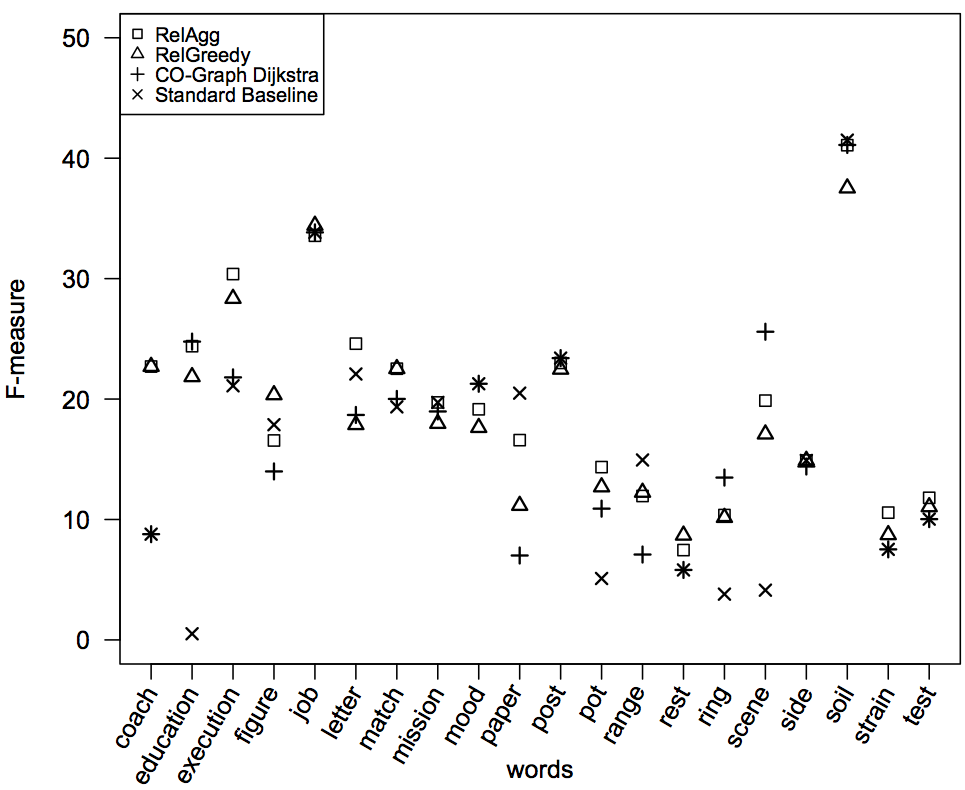
\includegraphics[width=0.5\textwidth]{plots/word-based-oof.png}
  \caption{Results of the \emph{OOF Result} evaluation based on each word using F-measure}
  \label{figure:wordresults-oof} 
\vspace{-0.7cm}
\end{figure}

The results for both the \emph{Out-Of-Five} and \emph{Best Result} evaluations show that our approach based on vector representation of the words outperforms the standard as well as the CO-Graph baselines. Comparing the relatedness approaches, we observe similar results for the RelAgg and RelGreedy methods, while RelAgg has slightly better performance, specially in the \emph{Best Result} evaluation. Regarding the different vector representations of the words with common evaluation and relatedness methods, we also see very similar results, while the GloVe method with 200 dimensions shows overall better performance.

In order to observe the effectiveness of the systems on different words, we selected the best performing settings in both RelAgg and RelGreedy (GloVe with 200 dimensions), and compared them with the standard and the CO-Graph baselines. The results for the \emph{Out-Of-Five} evaluation are shown in Figure~\ref{figure:wordresults-oof}\footnote{The corresponding plot for the \emph{Best Result} is available at supplementary-materials/evaluation}.

The results show that while for most words our approach outperforms the standard baseline as well as the CO-Graph system, none of the systems could outperform the standard baseline for ``mood'' and ``side''. Analyzing the evaluation results of these words, we observed that in some sentences, none of the nouns and verbs in the context share any common topic with senses of the ambiguous term. For example, using only the semantics of the nouns and verbs in the context, the correct sense of ``mood'' cannot be distinguished in either of the sentences: ``it reflected the \textit{mood} of the moment'' (state of the feeling) and ``a general \textit{mood} in Whitehall'' (inclination, tendency) . Similar cases were observed for the word ``side'': e.g., ``both \textit{sides} reaffirmed their commitment'' (groups opposing each other) in comparison to ``at the  \textit{side} of the cottage'' (a position to the left or right of a place). These examples show the limitations of the context-based methods. In addition to the context, the probability of occurrence of the words in a specific order (language modeling), potentially including terms of closed POS classes, is probably the missing piece here. 

\vspace{-0.3cm}

\section{Conclusion and Future Work}
\vspace{-0.3cm}
\label{sec:conclusion}
We study the opportunities of applying unsupervised approaches on CL-WSD, focusing on its application in English to Persian language. The proposed method  addresses the CL-WSD problem using semantic vector representations of the words in the context. In addition, addressing the problem of lack of standard evaluation framework for Persian language in the NLP domain, we create and make available a new benchmark for English to Persian CL-WSD following the format of the SemEval 2013 CL-WSD task. Finally, evaluating our approach on the new benchmark, we show that it outperforms both the CO-Graph system--a state-of-the-art system in unsupervised CL-WSD--as well as the standard baseline, for both the \emph{Best} and \emph{Out-of-five} evaluation metrics of the task.  

We have however also observed fundamental limitations of the methods based exclusively on context as bag of words. The combination of  language modeling and deep learning methods for CL-WSD will probably address these current limitations. Nevertheless, the current work offers a possible solution for all languages or domains with scarce knowledge-based  or parallel corpora resources, by exploiting the use of a monolingual corpus together with a bilingual lexicon.

% include your own bib file like this:
\bibliographystyle{acl}
\bibliography{refer}

\end{document}